\begin{figure}
  \centering
  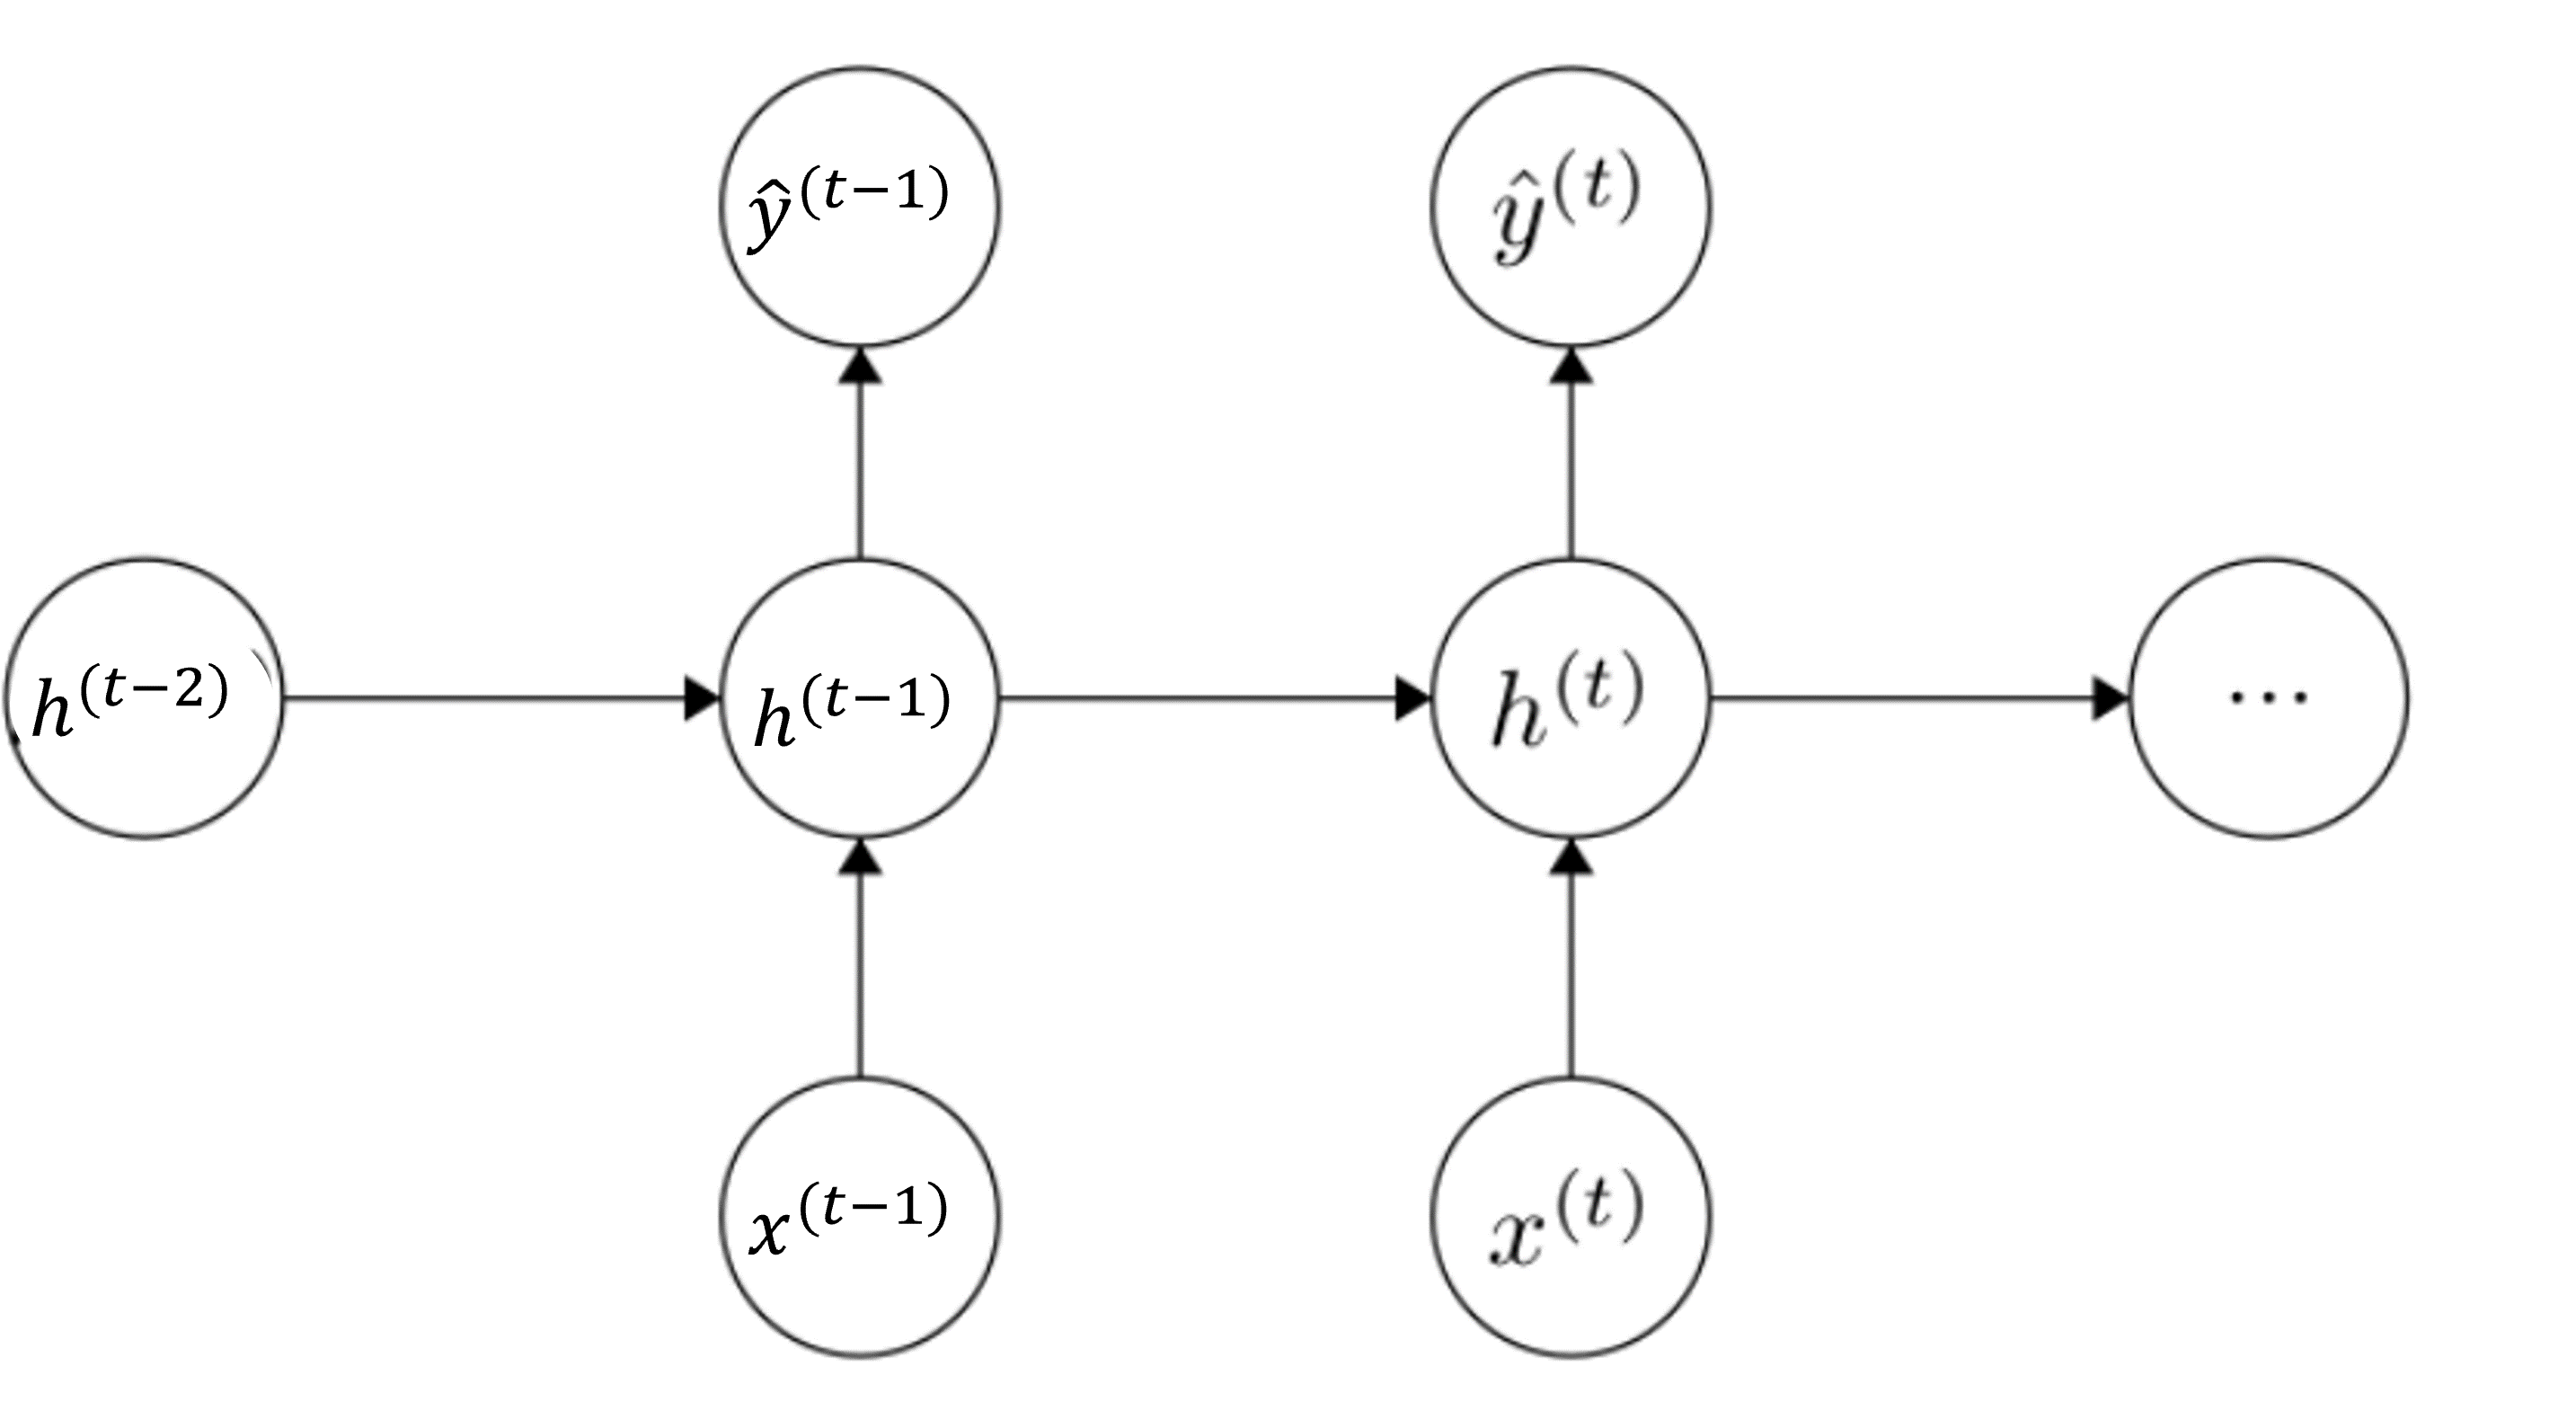
\includegraphics[width=0.9\linewidth]{q2/RNN_graph_updated.png}
  \label{fig:RNN_graph}
\end{figure}

We now backpropagate 1 step through time, expressing out answer using the terms requested in part (a).

\subsubsection[short]{$\frac{\partial J^{(t)}}{\partial L_{x^{(t-1)}}}(\theta)$}
Looking at equation (\ref{eq:grad_h_by_L}) shows us that:

\begin{equation} \label{eq:grad_h_by_L_induction_step}
  \begin{aligned}
    \frac{\partial h^{(t)}}{\partial L_{i,j}} &= \frac{\partial \sigma}{\partial a^{(t)}} \left( \frac{\partial}{\partial L_{i,j}} { \left(L_{x^{(t)}}I \right)}  + \frac{\partial }{\partial L_{i,j}} \left( {h^{(t-1)}}^T H \right) \right) \\
    &= \restr{\frac{\partial h^{(t)}}{\partial L_{i,j}}}{(t)} + \; \frac{\partial h^{(t)}}{\partial h^{(t-1)}} \cdot \frac{\partial h^{(t-1)}}{\partial L_{i,j}}
  \end{aligned}
\end{equation}

We can unroll one timestamp further into the past $(t-2)$ by applying the chain rule once again:
\begin{equation}
  \frac{\partial h^{(t-1)}}{\partial L_{i,j}} = \restr{\frac{\partial h^{(t-1)}}{\partial L_{i,j}}}{(t-1)} +\; \frac{\partial h^{(t-1)}}{\partial h^{(t-2)}} \cdot \frac{\partial h^{(t-2)}}{\partial L_{i,j}}
\end{equation}

Plugging this expression back into (\ref{eq:grad_h_by_L_induction_step}) gives:
\begin{equation}
  \begin{aligned}
    \frac{\partial h^{(t)}}{\partial L_{i,j}} &= \restr{\frac{\partial h^{(t)}}{\partial L_{i,j}}}{(t)} +\; \frac{\partial h^{(t)}}{\partial h^{(t-1)}} \left( \restr{\frac{\partial h^{(t-1)}}{\partial L_{i,j}}}{(t-1)} +\; \frac{\partial h^{(t-1)}}{\partial h^{(t-2)}} \cdot \frac{\partial h^{(t-2)}}{\partial L_{i,j}} \right) \\
    &= \restr{\frac{\partial h^{(t)}}{\partial L_{i,j}}}{(t)} +\; \frac{\partial h^{(t)}}{\partial h^{(t-1)}} \cdot \restr{\frac{\partial h^{(t-1)}}{\partial L_{i,j}}}{(t-1)} +\; \frac{\partial h^{(t)}}{\partial h^{(t-2)}} \cdot \frac{\partial h^{(t-2)}}{\partial L_{i,j}} \\
    &= \sum_{l=t-1}^{t}  \frac{\partial h^{(t)}}{\partial h^{(l)}} \cdot \restr{\frac{\partial h^{(l)}}{\partial L_{i,j}}}{(l)} \; + \; \frac{\partial h^{(t)}}{\partial h^{(t-2)}} \cdot \frac{\partial h^{(t-2)}}{\partial L_{i,j}}
  \end{aligned}
\end{equation}

Which using our notation yields:
\begin{equation}
  \begin{aligned}
    \frac{\partial J^{(t)}}{\partial L_{i,j}}(\theta) &= \sum_{l=t-1}^{t} \frac{\partial J^{(t)}}{\partial h^{(l)}} \cdot \restr{\frac{\partial h^{(l)}}{\partial L_{i,j}}}{(l)} \;+\; \frac{\partial J^{(t)}}{\partial h^{(t-2)}} \cdot \frac{\partial h^{(t-2)}}{\partial L_{i,j}} \\
    &= \sum_{l=t-1}^{t} \frac{\partial J^{(t)}}{\partial h^{(l)}} \cdot \restr{\frac{\partial h^{(l)}}{\partial L_{i,j}}}{(l)} \;+\; \frac{\partial J^{(t-2)}}{\partial L_{i,j}}
  \end{aligned}
\end{equation}

Substituting in for $\partial L_{x^{(t-1)}}$:
\begin{equation}
  \frac{\partial J^{(t)}}{\partial L_{x^{(t-1)}}}(\theta) = \sum_{l=t-1}^{t} \frac{\partial J^{(t)}}{\partial h^{(l)}} \cdot \restr{\frac{\partial h^{(l)}}{\partial L_{x^{(t-1)}}}}{(l)} \;+\; \frac{\partial J^{(t-2)}}{\partial L_{x^{(t-1)}}}
\end{equation}

where $\restr{\frac{\partial h^{(l)}}{\partial L_{x^{(t-1)}}}}{(l)} = 0$ whenever $x^{(l)} \neq x^{(t-1)}$. For simplicity, again assuming $x^{(t_1)} \neq x^{(t_2)}$ for any $t_1 \neq t_2$ gives:
\begin{equation}
    \boxed{ \frac{\partial J^{(t)}}{\partial L_{x^{(t-1)}}}(\theta) = \frac{\partial J^{(t)}}{\partial h^{(t-1)}} \cdot \restr{\frac{\partial h^{(t-1)}}{\partial L_{x^{(t-1)}}}}{(t-1)} }
\end{equation}

Or explicitly:
\begin{equation}
  \frac{\partial J^{(t)}}{\partial L_{x^{(t-1)}}}(\theta) = \left(\hat{y}^{(t)} - y^{(t)}\right)^T U^T \; \text{diag}\left[ h^{(t)} \right]  \text{diag}\left[ \vec{1} - h^{(t)} \right] H^T \text{diag}\left[ h^{(t-1)} \right]  \text{diag}\left[ \vec{1} - h^{(t-1)} \right] I^T 
\end{equation}


\subsubsection[short]{$\restr{\frac{\partial J^{(t)}}{\partial H}}{(t-1)}$}

By applying the same derivations such as in (\ref{eq:grad_h_by_H}):
\begin{equation}
  \begin{aligned}
    \restr{\frac{\partial J^{(t)}}{\partial H_{i,j}}}{(t-1)} &= \frac{\partial J^{(t)}}{\partial h^{(t-1)}} \cdot \restr{\frac{\partial h^{(t-1)}}{\partial H_{i,j}}}{(t-1)} \\
    &= \frac{\partial J^{(t)}}{\partial h^{(t-1)}} \cdot \text{diag}\left[ h^{(t-1)} \right]  \text{diag}\left[ \vec{1} - h^{(t-1)} \right] h^{(t-2)}_i \cdot \textbf{\text{e}}_j
  \end{aligned}
\end{equation}

which is reconized as the outer product:
\begin{equation}
  \boxed {\restr{\frac{\partial J^{(t)}}{\partial H}}{(t-1)} = h^{(t-2)} \otimes \left( \frac{\partial J^{(t)}}{\partial h^{(t-1)}} \cdot \text{diag}\left[ h^{(t-1)} \right]  \text{diag}\left[ \vec{1} - h^{(t-1)} \right] \right)^T }
\end{equation}

Or explicitly:
\begin{equation}
  \restr{\frac{\partial J^{(t)}}{\partial H}}{(t-1)} = h^{(t-2)} \otimes \left( \left(\hat{y}^{(t)} - y^{(t)}\right)^T U^T \; \text{diag}\left[ h^{(t)} \right]  \text{diag}\left[ \vec{1} - h^{(t)} \right] H^T \text{diag}\left[ h^{(t-1)} \right]  \text{diag}\left[ \vec{1} - h^{(t-1)} \right] \right)^T
\end{equation}


\subsubsection[short]{$\restr{\frac{\partial J^{(t)}}{\partial I}}{(t-1)}$}
In a similar fashion to the previous derivation:
\begin{equation}
  \boxed {\restr{\frac{\partial J^{(t)}}{\partial I}}{(t-1)} = e^{(t-1)} \otimes \left( \frac{\partial J^{(t)}}{\partial h^{(t-1)}} \cdot \text{diag}\left[ h^{(t-1)} \right]  \text{diag}\left[ \vec{1} - h^{(t-1)} \right] \right)^T }
\end{equation}


\subsubsection[short]{$\restr{\frac{\partial J^{(t)}}{\partial b_1}}{(t-1)}$}

\begin{equation}
  \begin{aligned}
    \restr{\frac{\partial J^{(t)}}{\partial b_1}}{(t-1)} &= \frac{\partial J^{(t)}}{\partial h^{(t-1)}} \cdot \restr{\frac{\partial h^{(t-1)}}{\partial b_1}}{(t-1)} \\
    &= \Aboxed{ \frac{\partial J^{(t)}}{\partial h^{(t-1)}} \cdot \text{diag}\left[ h^{(t-1)} \right]  \text{diag}\left[ \vec{1} - h^{(t-1)} \right] } 
  \end{aligned}
\end{equation}